
\chapter{Rezultaty}


\section{Testy wydajnościowe}
Po zakończeniu projektu przeprowadzono testy wydajnościowe aplikacji. Czas działania jednej iteracji naszej implementacji algorytmu kolonizacyjnego jest równy ${\Theta(n_i*m_i)}$, gdzie ${n_i}$ to liczba atraktorów
w danej iteracji, a ${m_i}$ to liczba węzłów w danej iteracji. Wynika on z konieczności wyznaczenia dla każdego atraktora najbliższego węzła drzewa.
Ciężko jest określić liczbę iteracji algorytmu potrzebnych do zakończenia, gdyż zależy ona równocześnie od kilku parametrów algorytmu.
 Na wykresie widzimy
szybki początkowy wzrost czasu potrzebnego na wygenerowanie modelu, a następnie zmianę szybkości wzrostu. Wynika ona z ograniczonej ilości
pamięci dostępnej dla procedury generowania, ustalonej by czas generowania drzewa dla dowolnej liczby atraktorów nie przekroczył kilkunastu sekund.



\begin{center}
	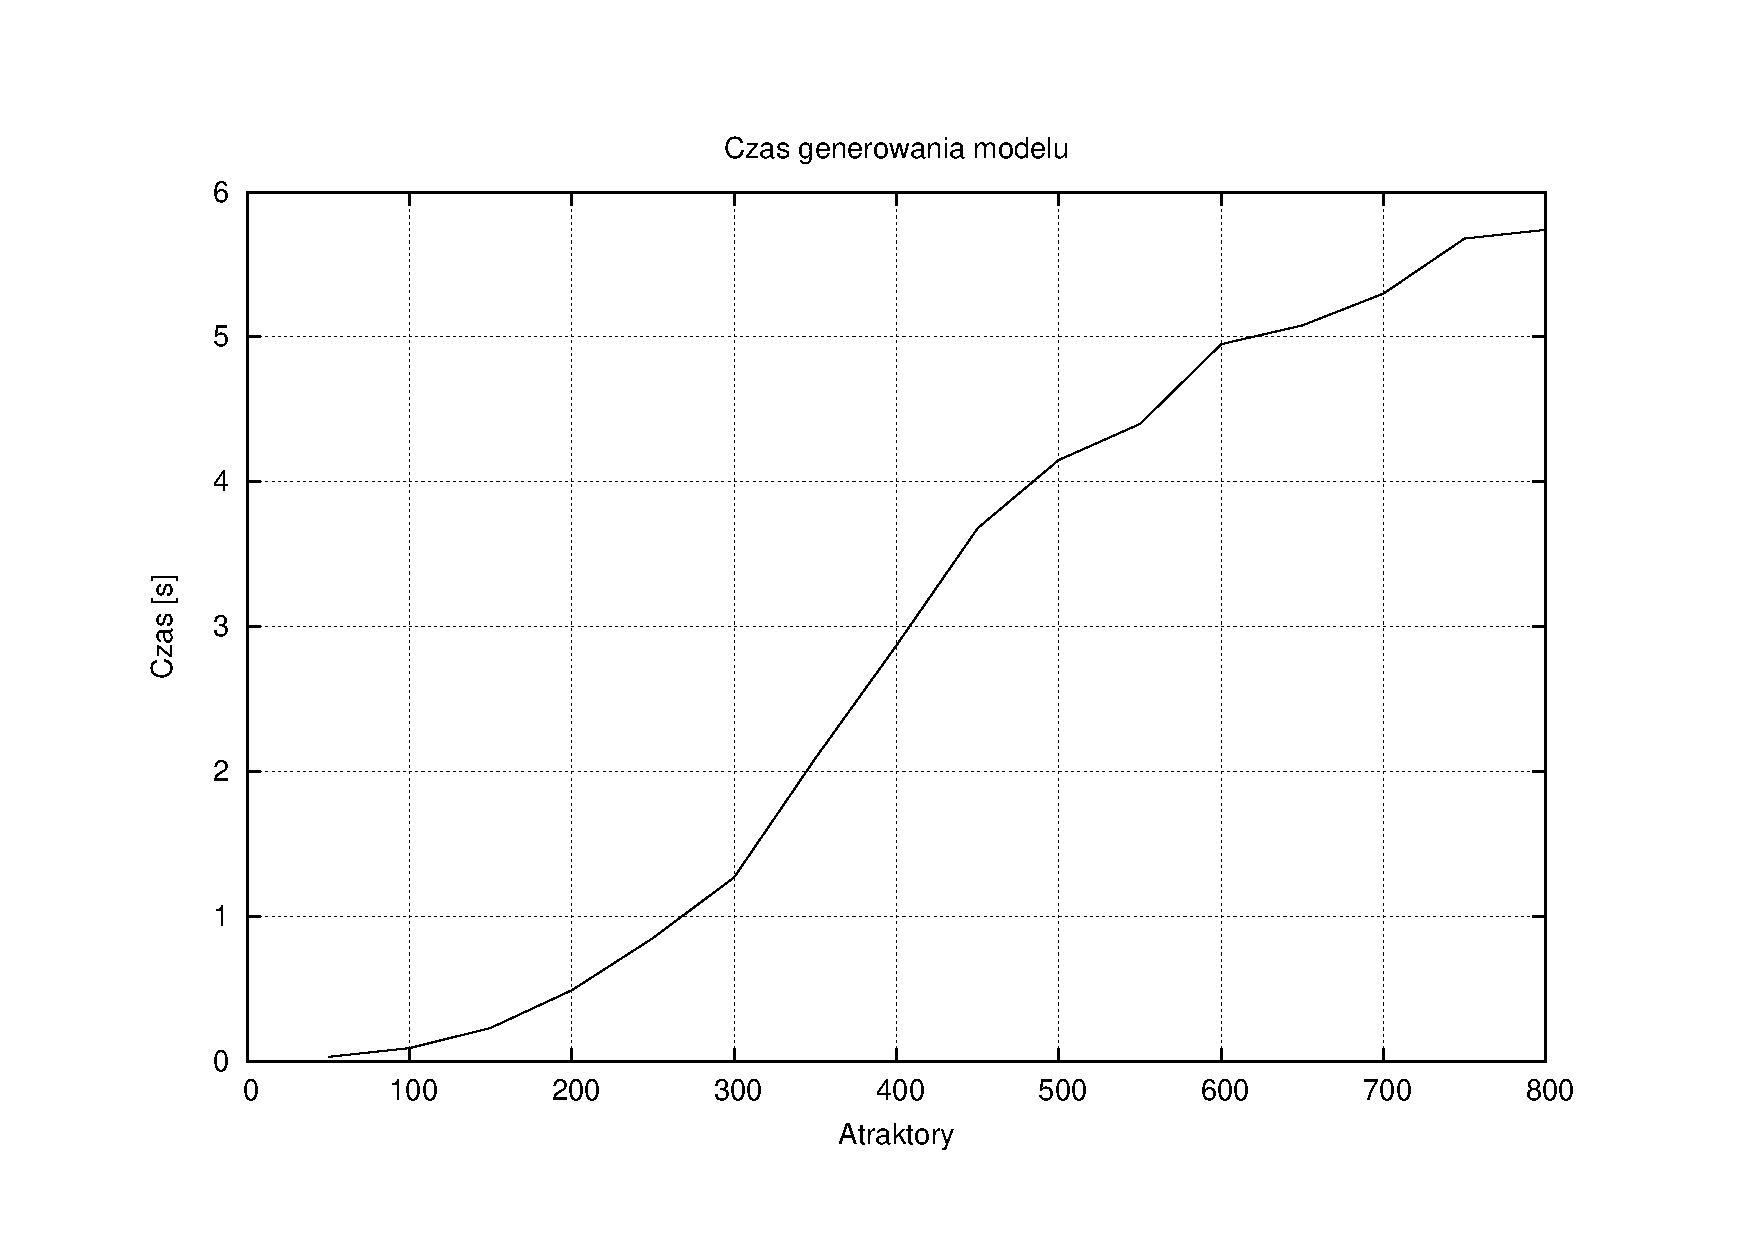
\includegraphics[width=90mm]{images/performance.pdf}
	\captionof{figure}{Czas generowania modelu w zależności od liczby atraktorów.}
\end{center}

\section{Ostateczny wygląd aplikacji}
\begin{center}
	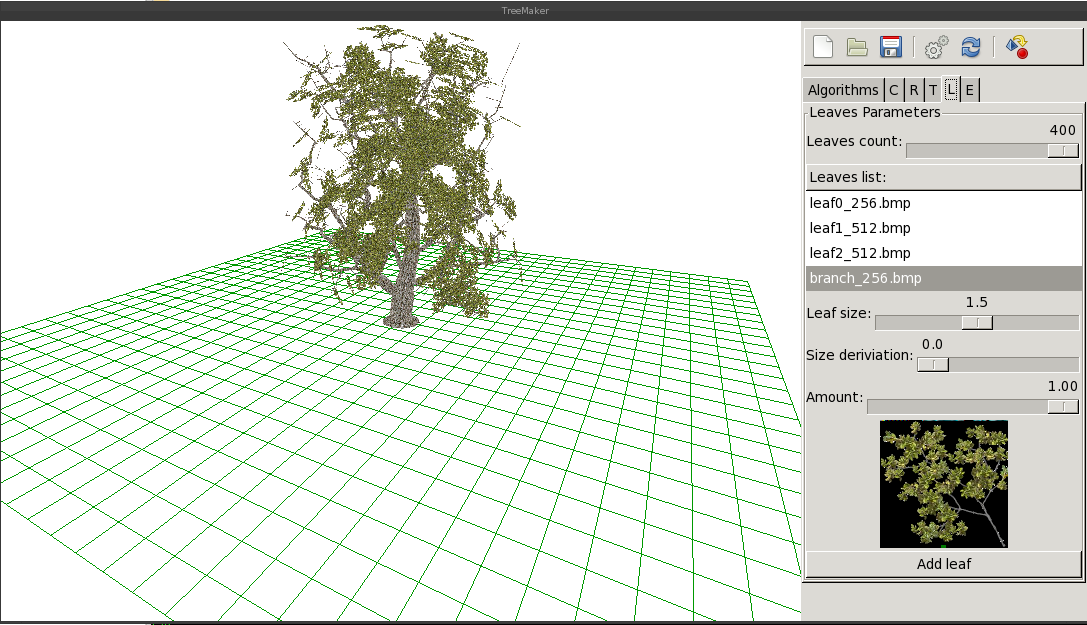
\includegraphics[width=120mm]{images/gui/all.png}
	\captionof{figure}{Wygląd aplikacji.}
\end{center}

\section{Przykładowe modele drzew}
Poniżej przedstawiono przykładowe modele drzew, wraz z opisem głównych parametrów wpływających na ich ostateczny wygląd.
Wszystkie obrazy zostały utworzone przez program Blender. Więcej uzyskanych obrazów znajduje się na dołączonej płycie CD.
\begin{center}
	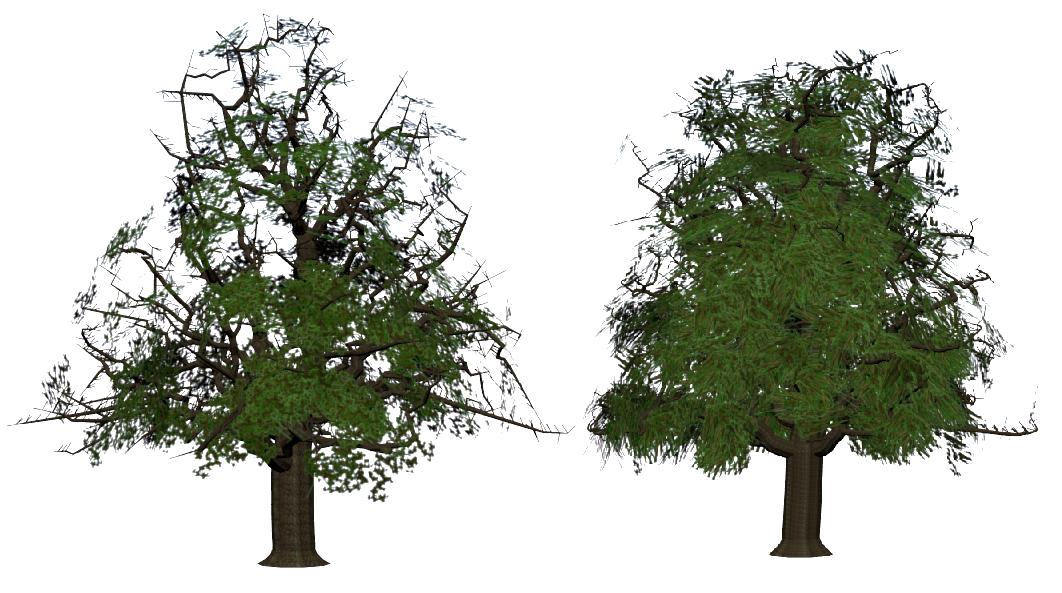
\includegraphics[width=100mm]{images/renders/greentree.png}
	\captionof{figure}{Wpływ liczby liści na wygląd drzewa}
\end{center}

\begin{center}
	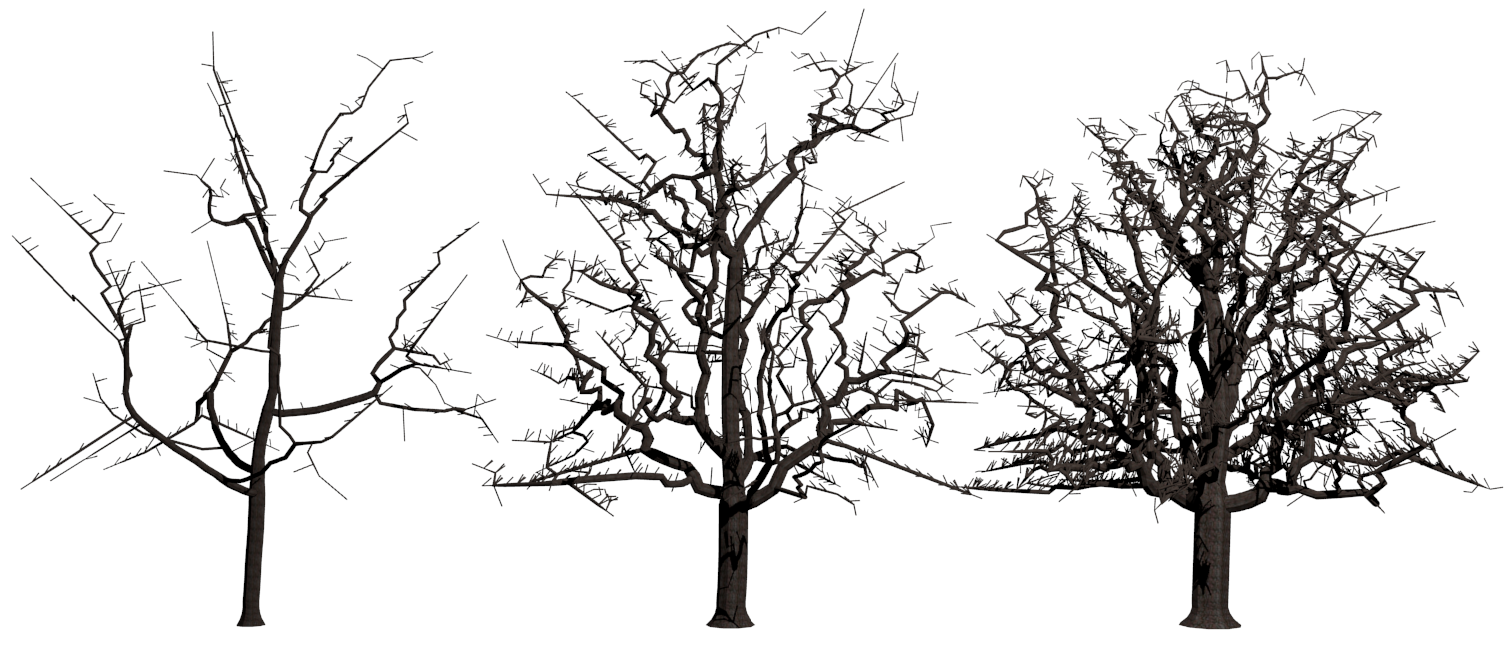
\includegraphics[width=120mm]{images/renders/points.png}
	\captionof{figure}{Wpływ liczby atraktorów na wygląd drzewa}
\end{center}

\begin{center}
	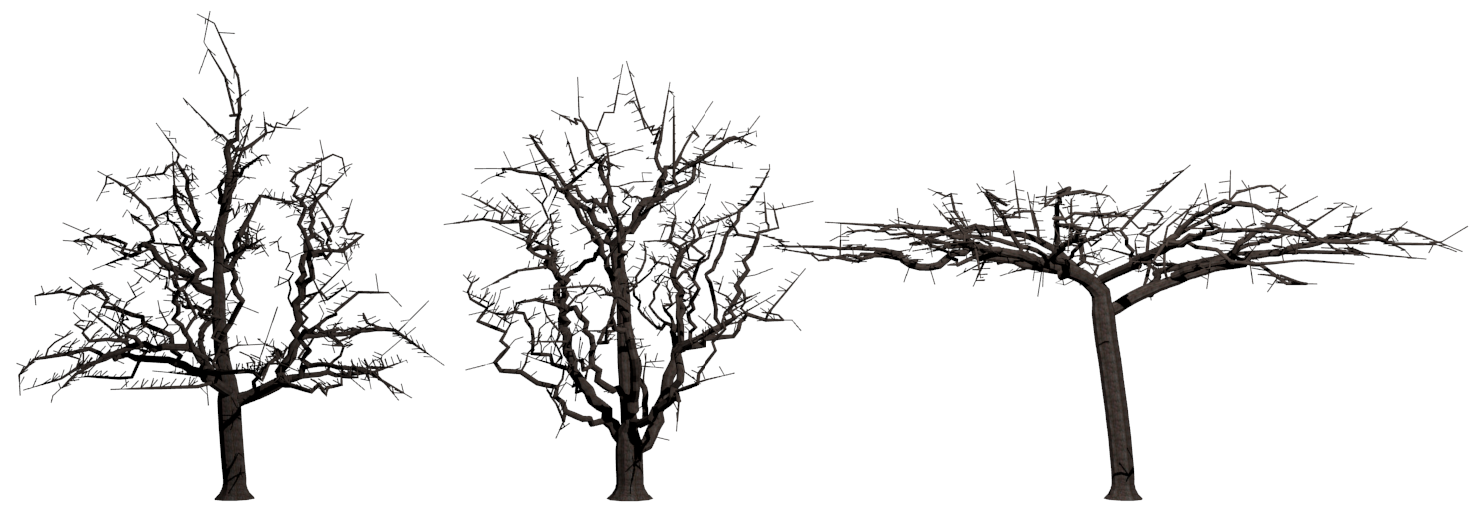
\includegraphics[width=120mm]{images/renders/shape.png}
	\captionof{figure}{Wpływ kształtu korony na wygląd drzewa}
\end{center}

\begin{center}
	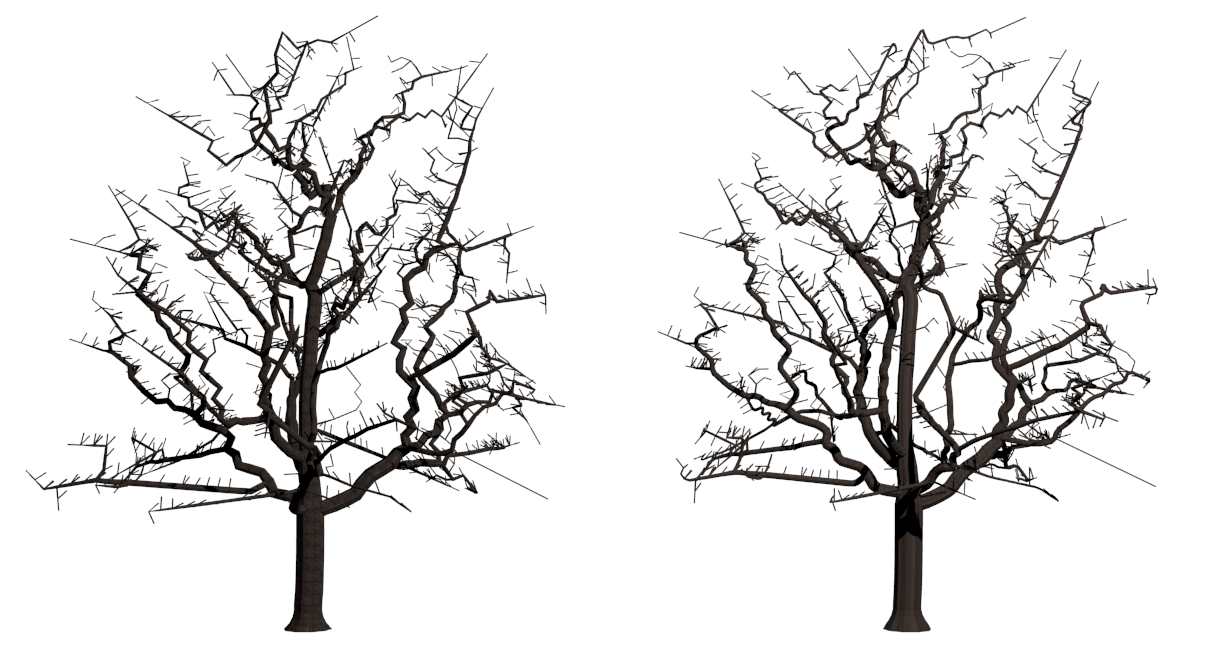
\includegraphics[width=120mm]{images/renders/smooth.png}
	\captionof{figure}{Wpływ wygładzania gałęzi na wygląd drzewa}
\end{center}


